\section{Results}
\subsection{Fairness Analysis on Tabular Data}
In the context of the work done on the Folktables, we decided to explore the profiles for which the XAI explanations were showing gendered anchors or gendered SHAP values. To move beyond a purely tabular analysis and gain a holistic, spatial understanding of these profiles, we employed a classic dimensionality reduction technique.

For this purpose, we applied Principal Component Analysis (PCA) \cite{pca-mackiewicz} with 2 components to the test dataset. This technique projects the high-dimensional feature space onto a two-dimensional plane defined by the principal components that capture the maximum variance within the data. This projection is crucial as it allows us to:

\begin{itemize}
    \item Assess Data Consistency: Compare the distributions of the training and test sets to ensure the stability and representativeness of our analysis, guarding against artifacts caused by data drift.

    \item Visualize Complex Relationships: See how individuals are spatially distributed based on their combined socioeconomic and demographic characteristics (e.g., age, education, occupation, marital status, ...).
    
    \item Identify Macro-Groups: Observe if individuals with similar XAI explanation patterns (e.g., gendered anchors) naturally coalesce into distinct groups within this reduced space, suggesting underlying demographic substructures that the model is drawing.
\end{itemize}


Figure \ref{fig:pca_tx} show the PCA of the Texas state made for four configurations. Model trained with XGBoost or HistGradientBoosting and explained with the Anchors or SHAP method.
On the left we have the test data in contrast to the training data, confirming no significant discrepancy, and on the right the PCA of the test data in contrast with the gendered explanation found within it. The PCA applied on test data of California and New York can be found in Figures \ref{fig:pca_ca} and \ref{fig:pca_ny}. Applying the PCA is a first step to see where the gendered explanations are concentrated and how each XAI method draw it.

\begin{figure}[h]
    \centering
    \begin{subfigure}[b]{0.9\textwidth}
        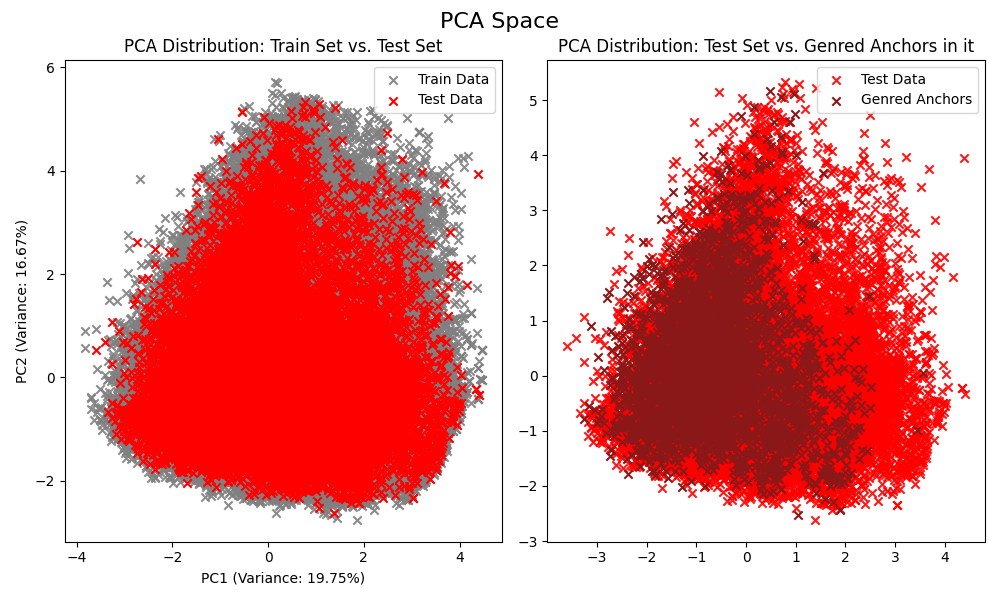
\includegraphics[width=\textwidth]{Images/pca/pca_xg_ca_anchors.png}
        \caption{Model: XGBoost, XAI method: Anchors}
        \label{fig:pca_xg_ca_anchors}
    \end{subfigure}
    \hfill
    \begin{subfigure}[b]{0.9\textwidth}
        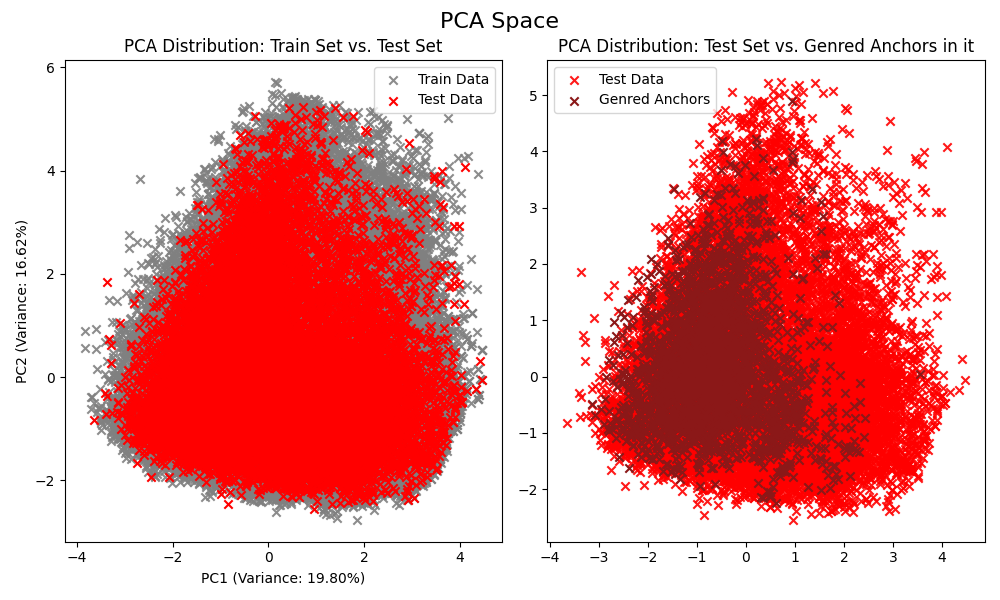
\includegraphics[width=\textwidth]{Images/pca/pca_skrub_ca_anchors.png}
        \caption{Model: HistGradientBoosting, XAI method: Anchors}
        \label{fig:pca_skrub_ca_anchors}
    \end{subfigure}
    \caption{PCA of the test dataset in the California state (Part 1)}
 \end{figure}

\begin{figure}[h]
    \ContinuedFloat
    \begin{subfigure}[b]{0.9\textwidth}
        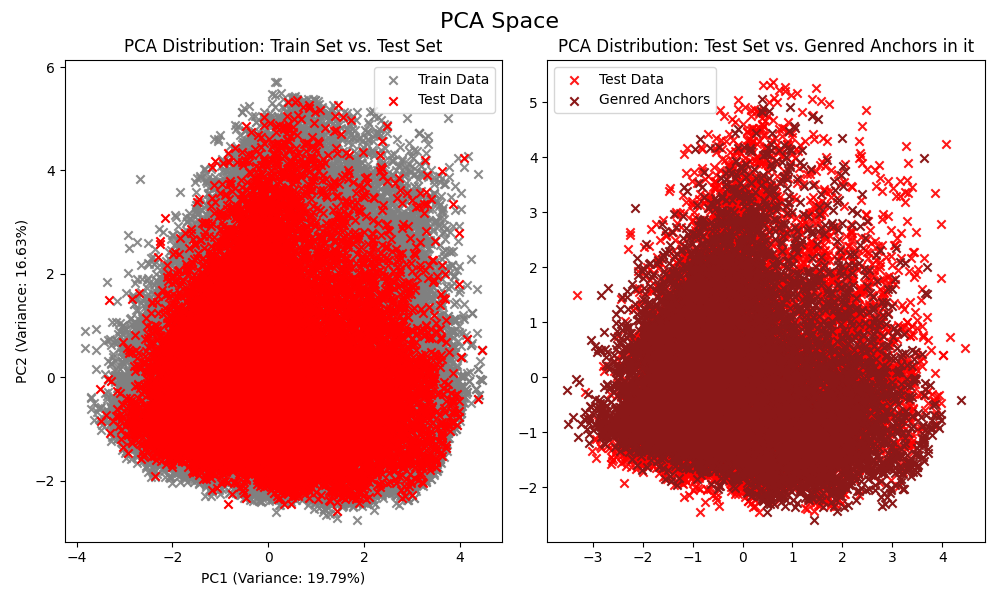
\includegraphics[width=\textwidth]{Images/pca/pca_xg_ca_shap.png}
        \caption{Model: XGBoost, XAI method: SHAP}
        \label{fig:pca_xg_ca_shap}
    \end{subfigure}
    \hfill
    \begin{subfigure}[b]{0.9\textwidth}
        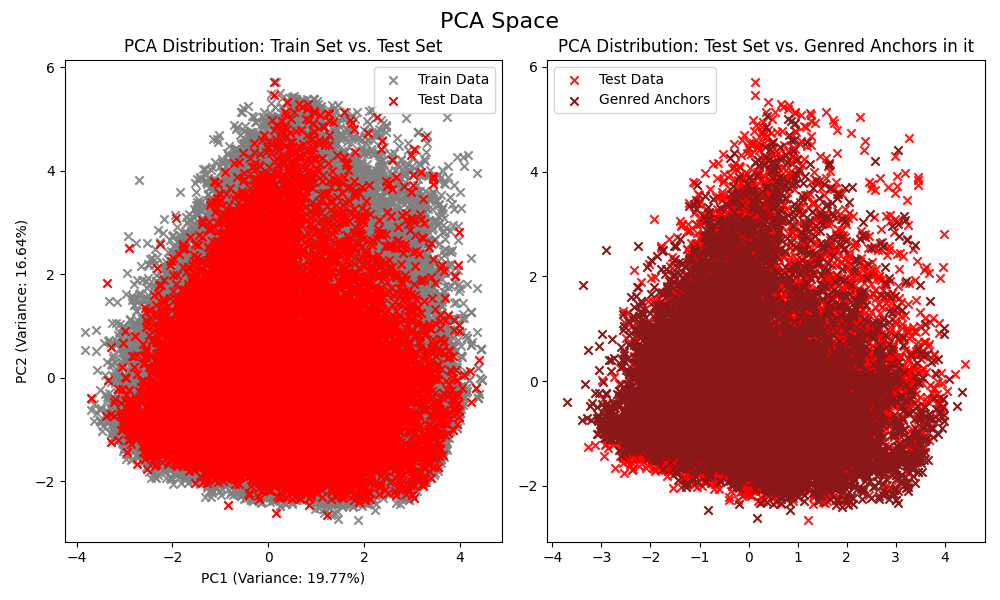
\includegraphics[width=\textwidth]{Images/pca/pca_skrub_ca_shap.png}
        \caption{Model: HistGradientBoosting, XAI method: SHAP}
        \label{fig:pca_skrub_ca_shap}
    \end{subfigure}
    \caption{PCA of the test dataset in the California state (Part 2)}
    \label{fig:pca_ca}
\end{figure}
    


\begin{figure}[h]
    \centering
    \begin{subfigure}[b]{0.9\textwidth}
        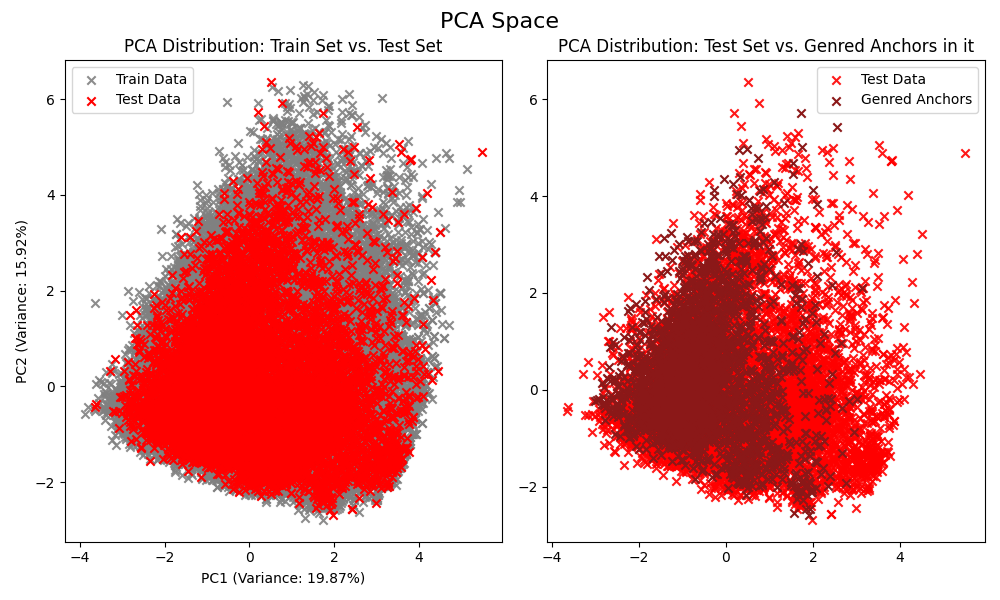
\includegraphics[width=\textwidth]{Images/pca/pca_xg_ny_anchors.png}
        \caption{Model: XGBoost, XAI method: Anchors}
        \label{fig:pca_xg_ny_anchors}
    \end{subfigure}
    \hfill
    \begin{subfigure}[b]{0.9\textwidth}
        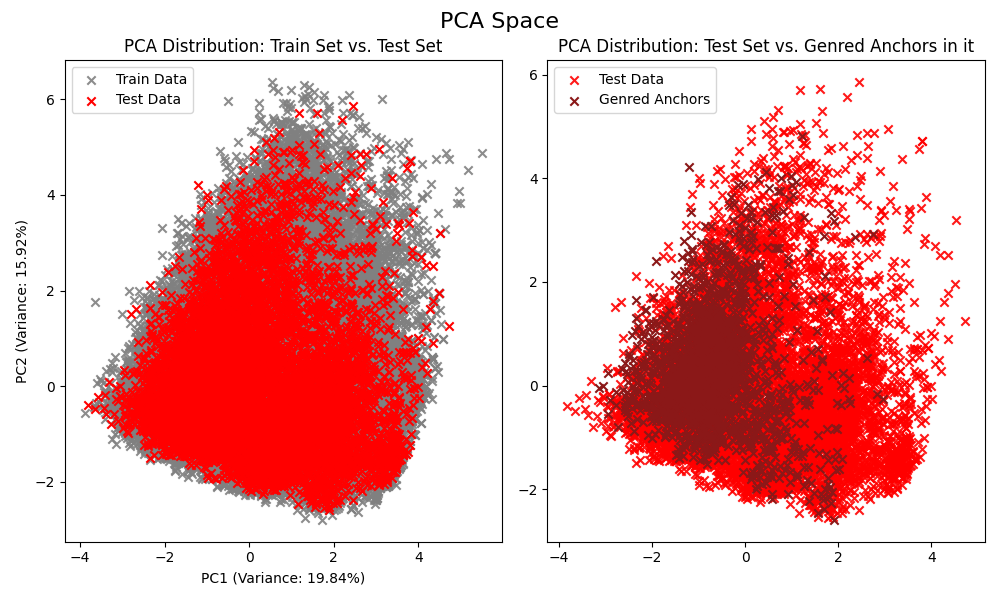
\includegraphics[width=\textwidth]{Images/pca/pca_skrub_ny_anchors.png}
        \caption{Model: HistGradientBoosting, XAI method: Anchors}
        \label{fig:pca_skrub_ny_anchors}
    \end{subfigure}
\caption{PCA of the test dataset in the New York state (Part 1)}
 \end{figure}

\begin{figure}[h]
    \ContinuedFloat
    \begin{subfigure}[b]{0.9\textwidth}
        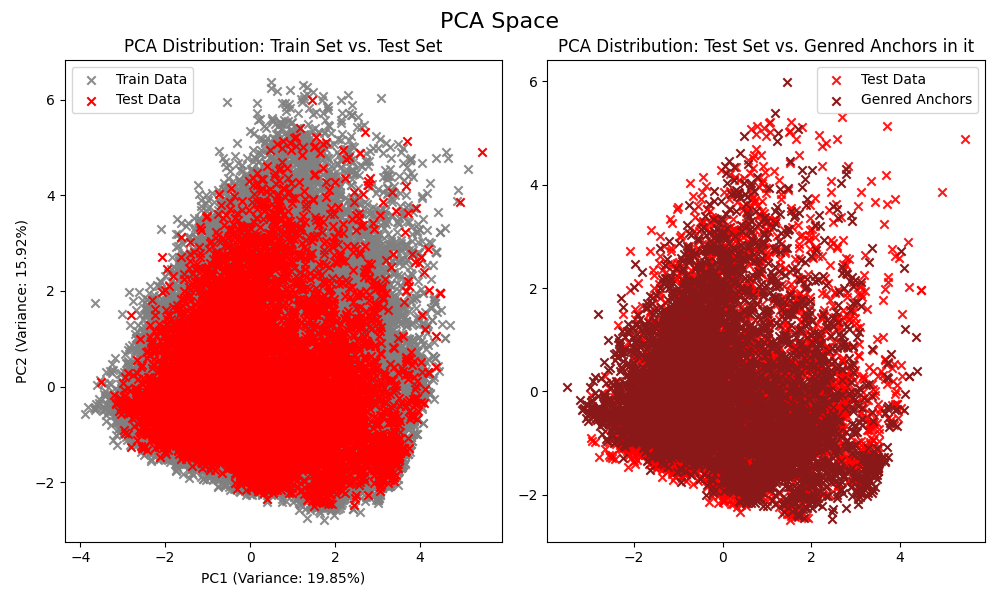
\includegraphics[width=\textwidth]{Images/pca/pca_xg_ny_shap.png}
        \caption{Model: XGBoost, XAI method: SHAP}
        \label{fig:pca_xg_ny_shap}
    \end{subfigure}
    \hfill
    \begin{subfigure}[b]{0.9\textwidth}
        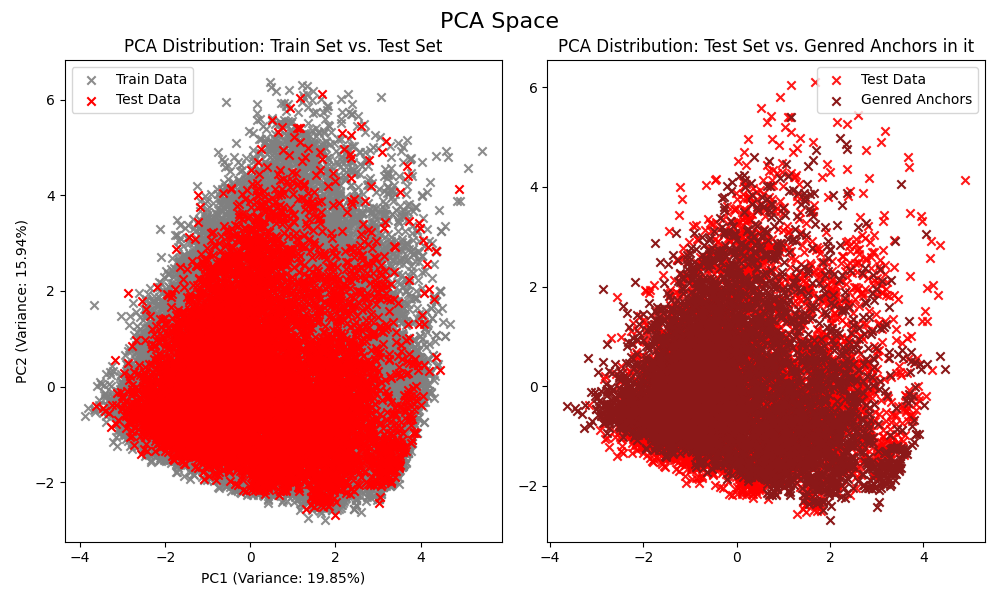
\includegraphics[width=\textwidth]{Images/pca/pca_skrub_ny_shap.png}
        \caption{Model: HistGradientBoosting, XAI method: SHAP}
        \label{fig:pca_skrub_ny_shap}
    \end{subfigure}
    \caption{PCA of the test dataset in the New York state (Part 2)}
    \label{fig:pca_ny}
\end{figure}

The next step is to formally define and label the distinct profiles observed in the PCA projection, we subsequently applied K-means clustering with three clusters \cite{kmeans-pca-ding}. This classic technique complements the PCA by algorithmmatically identifying dense regions of data points, thus quantitatively defining the macro-groups suggested by the visual inspection. This two-step approach—unsupervised projection followed by clustering—provides a robust, data-driven foundation for interpreting the XAI results. It allows us to move from observing vague groupings to analyzing well-defined clusters, each representing a specific demographic and socioeconomic profile prevalent in the data.

In Figure \ref{fig:clusters_tx} we can see the clustered PCA with the same configurations used in the figures described in Section \ref{met:fairness-xai}. The clustered PCA applied to the test data of California and New York can be found in Figures \ref{fig:clusters_ca} and \ref{fig:clusters_ny}.

\begin{figure}[h]
    \centering
    \begin{subfigure}[b]{1.0\textwidth}
        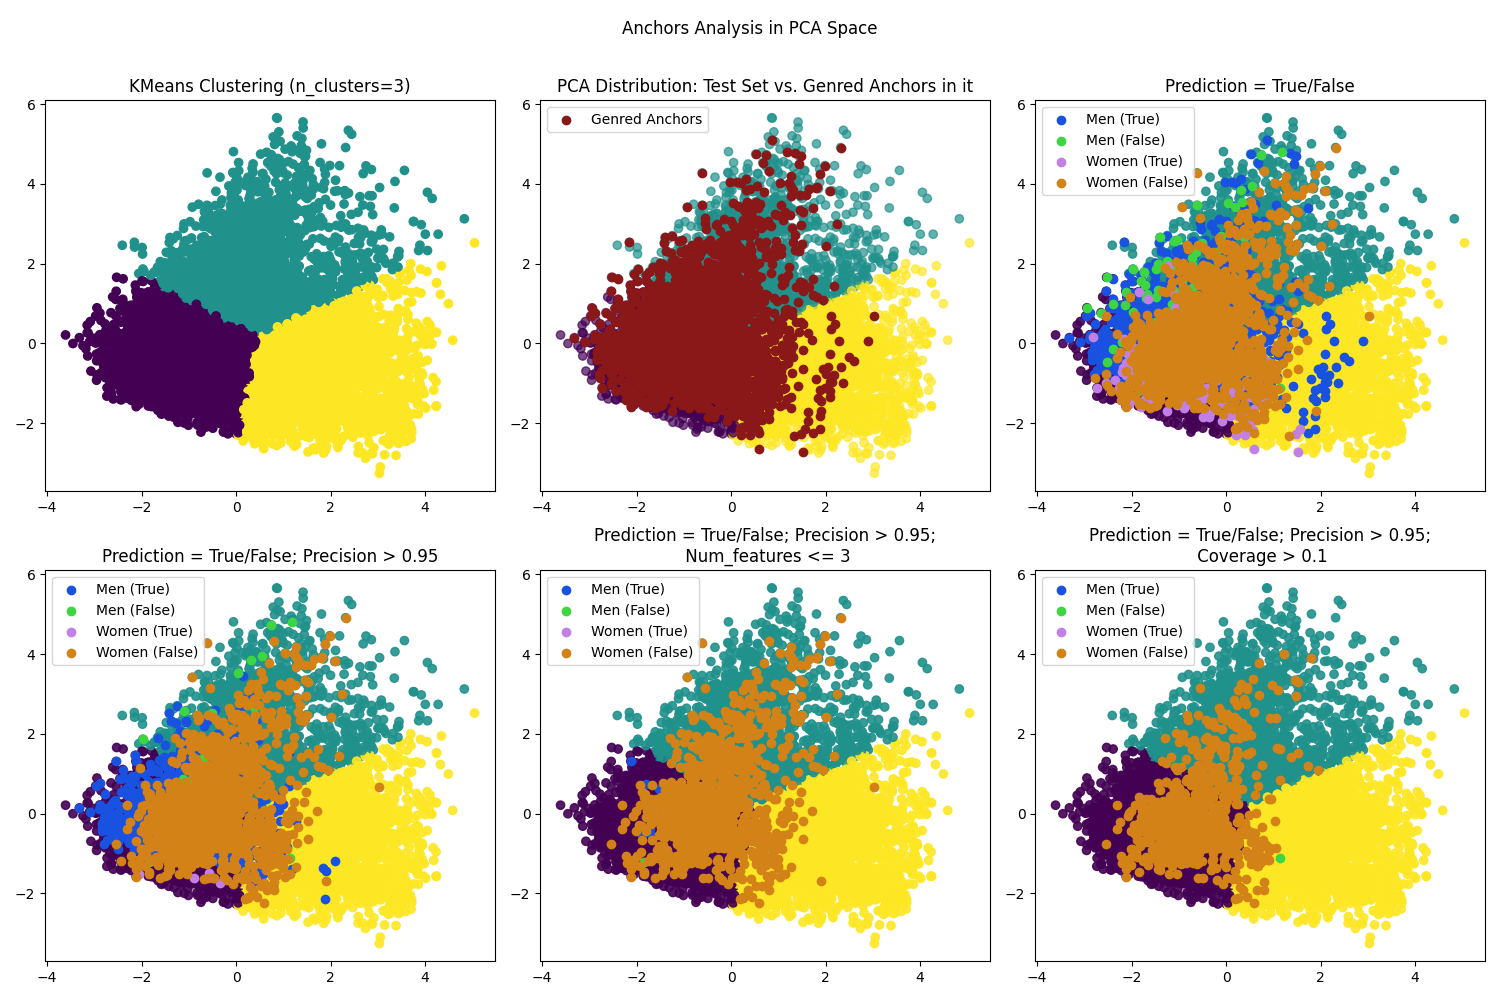
\includegraphics[width=\textwidth]{Images/clustered_pca/clusters_xg_tx_anchors.png}
        \caption{Model: XGBoost, XAI method: Anchors}
        \label{fig:clusters_xg_tx_anchors}
    \end{subfigure}

    \begin{subfigure}[b]{1.0\textwidth}
        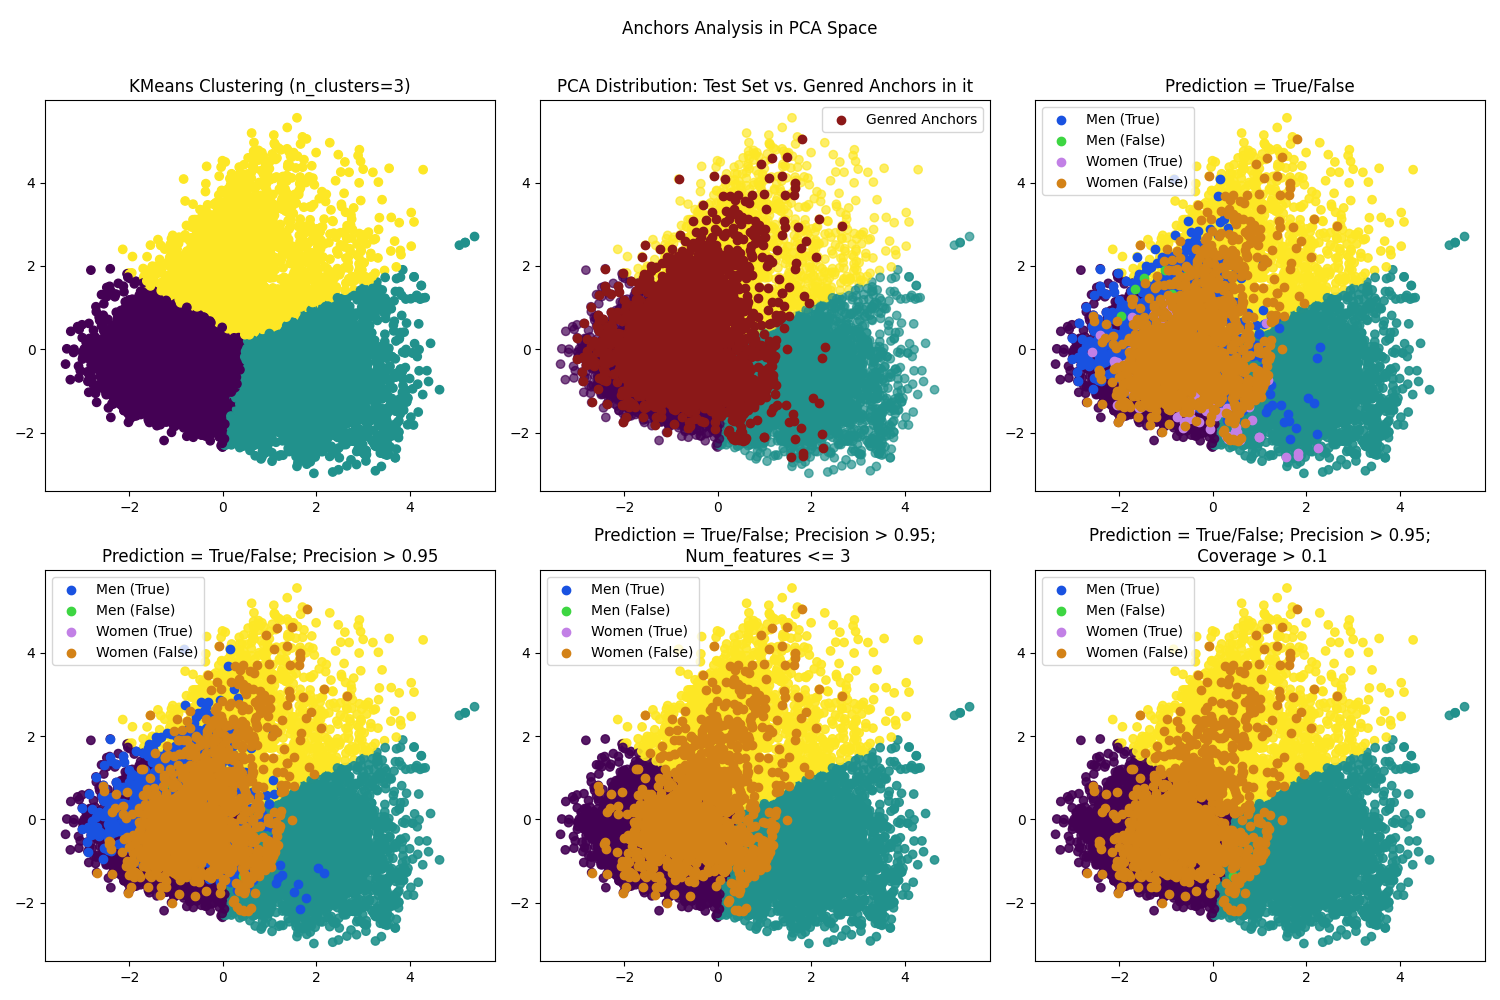
\includegraphics[width=\textwidth]{Images/clustered_pca/clusters_skrub_tx_anchors.png}
        \caption{Model: HistGradientBoosting, XAI method: Anchors}
        \label{fig:clusters_skrub_tx_anchors}
    \end{subfigure}
    \caption{Comparison of the clustered PCA in the Texas state, putting in evidence gendered explanations (Part 1)}
\end{figure}

\begin{figure}[h]
    \ContinuedFloat
    \begin{subfigure}[b]{1.0\textwidth}
        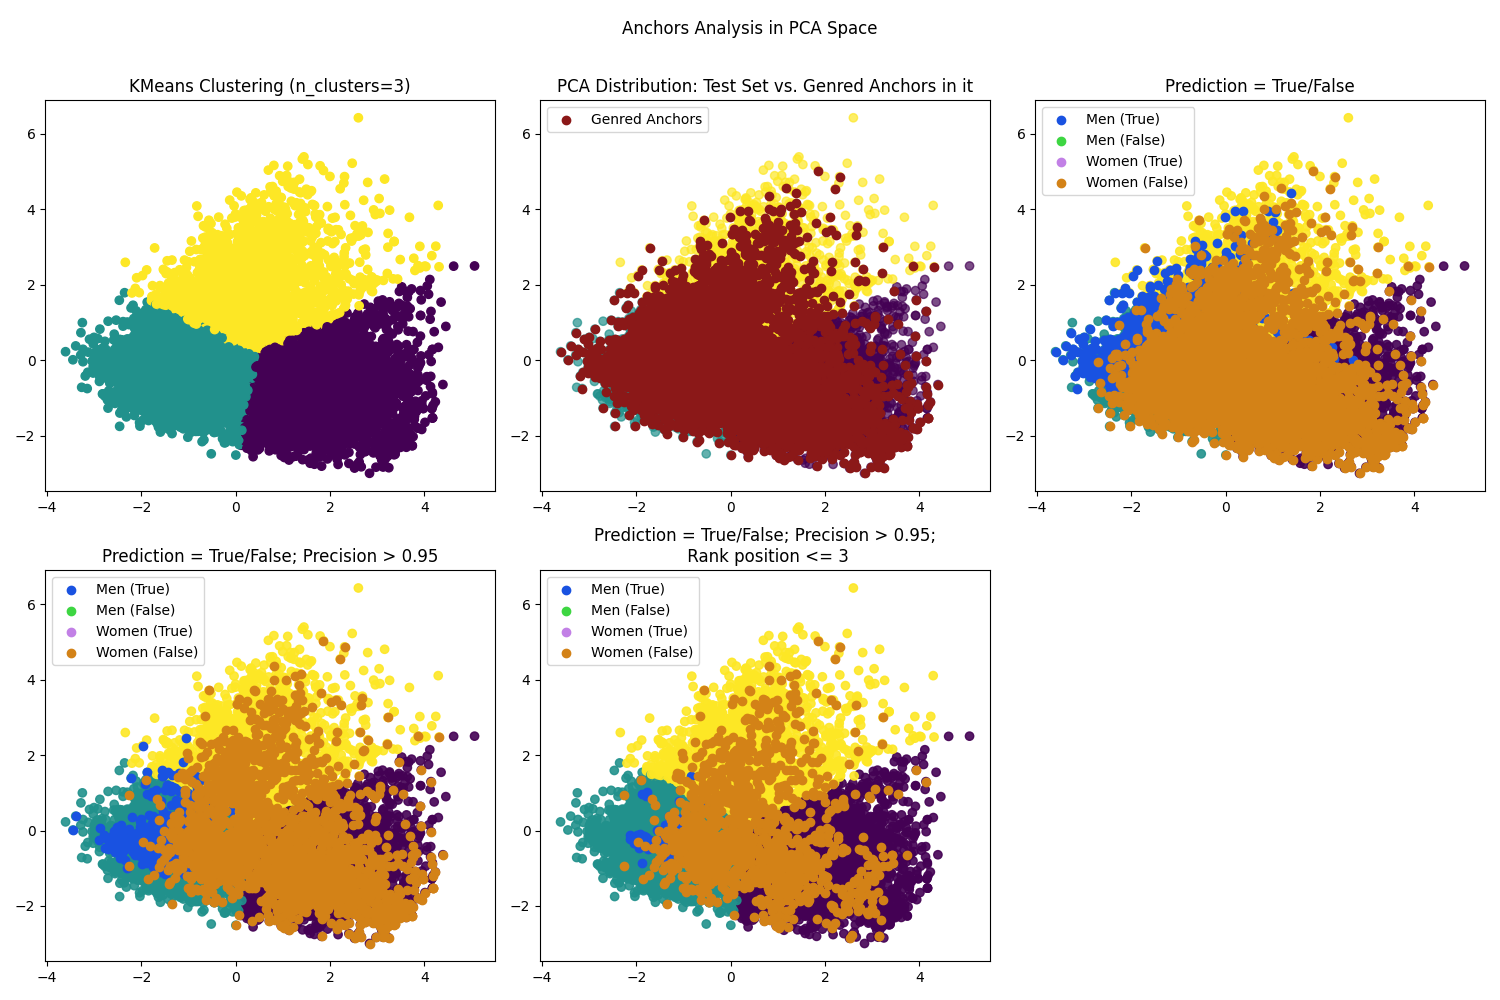
\includegraphics[width=\textwidth]{Images/clustered_pca/clusters_xg_tx_shap.png}
        \caption{Model: XGBoost, XAI method: SHAP}
        \label{fig:clusters_xg_tx_shap}
    \end{subfigure}

    \begin{subfigure}[b]{1.0\textwidth}
        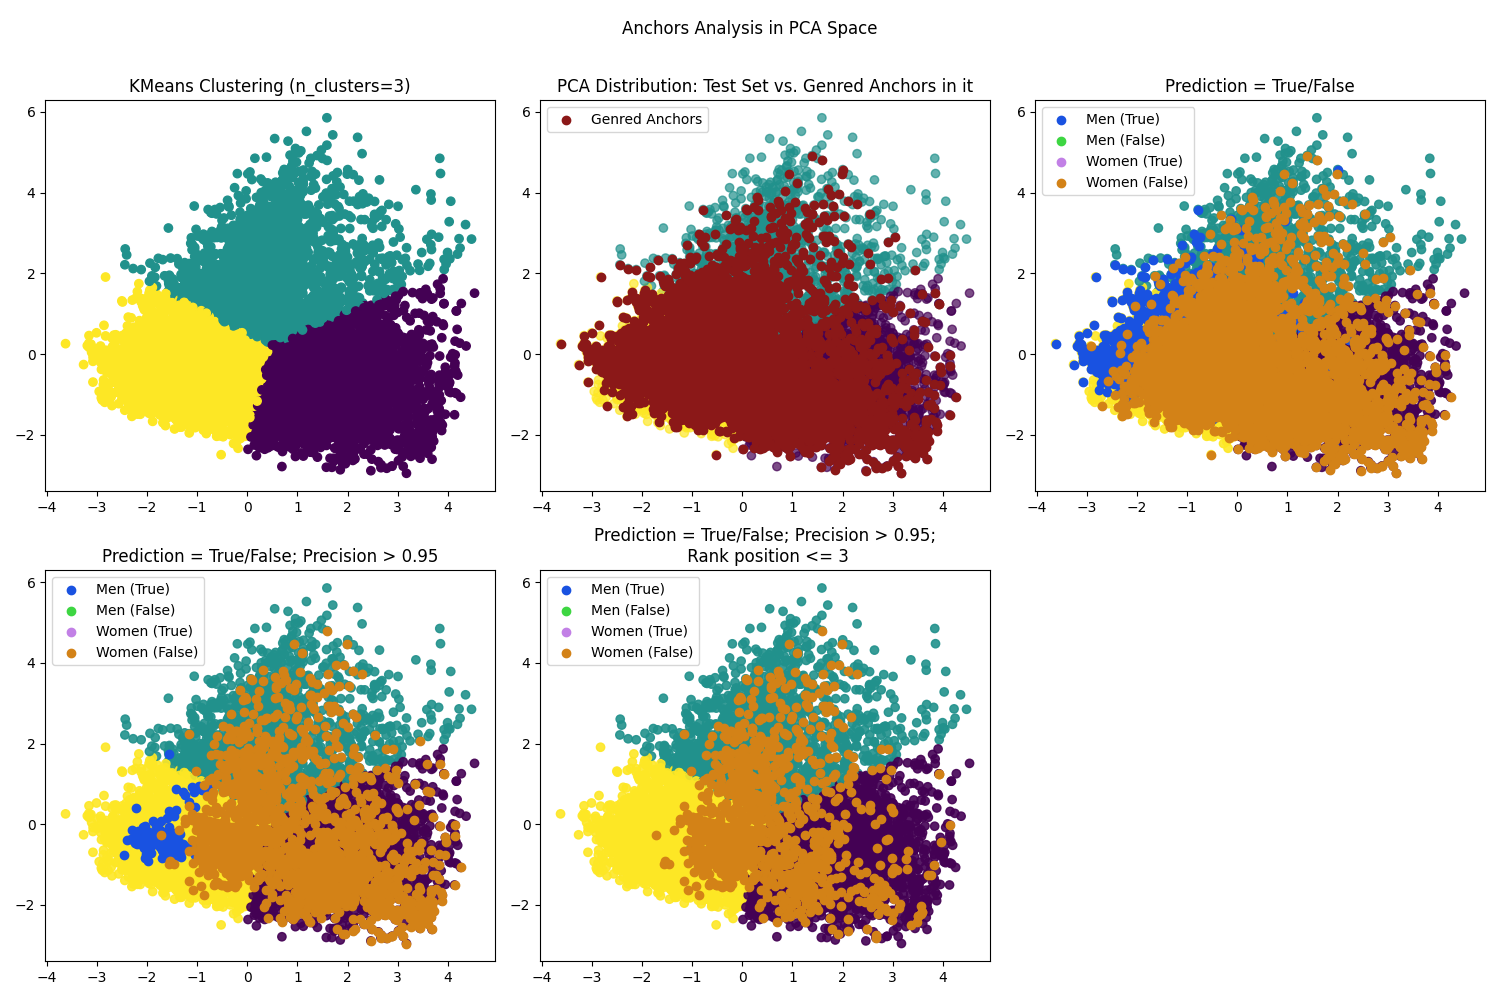
\includegraphics[width=\textwidth]{Images/clustered_pca/clusters_skrub_tx_shap.png}
        \caption{Model: HistGradientBoosting, XAI method: SHAP}
        \label{fig:clusters_skrub_tx_shap}
    \end{subfigure}

    \caption{Comparison of the clustered PCA in the Texas state, putting in evidence gendered explanations (Part 2)}
    \label{fig:clusters_tx}
\end{figure}

Figures \ref{fig:clusters_xg_tx_anchors} and \ref{fig:clusters_skrub_tx_anchors} build for the Anchors XAI method are organized as follows:
\begin{enumerate}
    \item KMeans clustering with 3 clusters of the PCA of test data
    \item Contrast of the gendered anchors with the clustering of the PCA
	\item Contrast of gendered anchors with the clustering organized by category (Men with true predictions, en with False predictions, Women with true predictions and Women with false predictions)
	\item Contrast of gendered anchors with the clustering organized by category, and filtering the anchors with a precision higher than 95\%.
	\item Contrast of gendered anchors with the clustering organized by category, and filtering the anchors with a precision higher than 95\% and a rule size limited to three features (meaning a compact anchor).
	\item Contrast of gendered anchors with the clustering organized by category, and filtering the anchors with a precision higher than 95\% and coverage of the anchors higher than 10\% of the dataset.
\end{enumerate}

Figures \ref{fig:clusters_xg_tx_shap} and \ref{fig:clusters_skrub_tx_shap} build for the SHAP XAI method are organized as follows:
\begin{enumerate}
    \item KMeans clustering with 3 clusters of the PCA of test data
    \item Contrast of the gendered SHAP values with the clustering of the PCA
	\item Contrast of gendered SHAP values with the clustering organized by category (Men with true predictions, en with False predictions, Women with true predictions and Women with false predictions)
	\item Contrast of gendered SHAP values with the clustering organized by category, and filtering the predictions with a precision higher than 95\%.
	\item Contrast of gendered SHAP values with the clustering organized by category, and filtering the predictions with a precision higher than 95\% and the SHAP values in which the 'SEX' variable is in the top 3 of the ranking.
\end{enumerate}

The code for all this analysis and results was developed to be a Python library and can be found in the GitHub repository \cite{fairness-experiments}.

\FloatBarrier

%%%%%%%%%%%%%%%%%%%%%%%%%%%%%%%%%%%%%%%%%%%%%%%%%%%%%%%%%%%%%%%%%%%%%%%%%%%%%%%%%%%%%%%%%%%%%%%%%%%%%%%%%%%%%%%%%%%%%%%
%%%%%%%%%%%%%%%%%%%%%%%%%%%%%%%%%%%%%%%%%%%%%%%%   MÉTÉO   %%%%%%%%%%%%%%%%%%%%%%%%%%%%%%%%%%%%%%%%%%%%%%%%%%%%%%%%%%%%
%%%%%%%%%%%%%%%%%%%%%%%%%%%%%%%%%%%%%%%%%%%%%%%%%%%%%%%%%%%%%%%%%%%%%%%%%%%%%%%%%%%%%%%%%%%%%%%%%%%%%%%%%%%%%%%%%%%%%%%

\subsection{"Anchors Regression" applied on Meteorological Data}
Given the methodology previously exposed, we constructed our solution using the framework of \textit{py4cast}.
Based on the objective of rain prediction, we prioritized a subset of channels to simplify the initial problem complexity. We built a more controlled environment with only three channels, the ones most directly associated with the physics of rainfall in the lower atmosphere, such as:
\begin{itemize}
	\item \textit{aro\_tp\_0m} (Total Precipitation)
	\item \textit{aro\_u10\_10m} (Zonal wind component at 10m)
    \item \textit{aro\_v10\_10m} (Meridional wind component at 10m)
\end{itemize}

In that way, we could test the approach with simpler data and adapt the hyperparameters before progressing to models using twenty channels.

Figure \ref{fig:titan-rain-perturbations} shows examples of how we perturb the channels with the masks for each one of the three channels to generate the counterfactuals.

\begin{figure}[h]
    \centering
    \begin{subfigure}[b]{0.32\textwidth}
        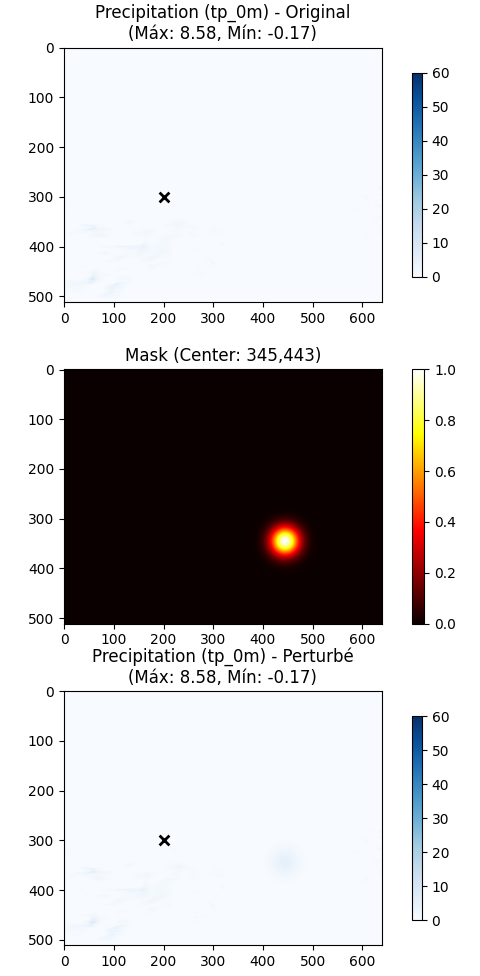
\includegraphics[width=\textwidth]{Images/titan_rain_perturbations/perturbed_c_tp_0m.png}
        \caption{Channel aro\_tp\_0m}
        \label{fig:titan_perturbed_aro_tp}
    \end{subfigure}
    \hfill
    \begin{subfigure}[b]{0.32\textwidth}
        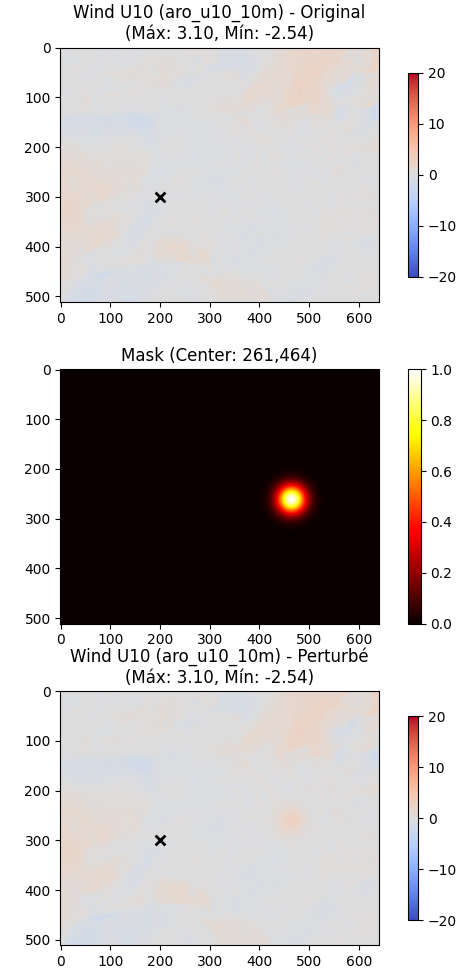
\includegraphics[width=\textwidth]{Images/titan_rain_perturbations/perturbed_c_u10_10m.png}
        \caption{Channel aro\_u10\_10m}
        \label{fig:titan_perturbed_aro_u10}
    \end{subfigure}
    \hfill
    \begin{subfigure}[b]{0.32\textwidth}
        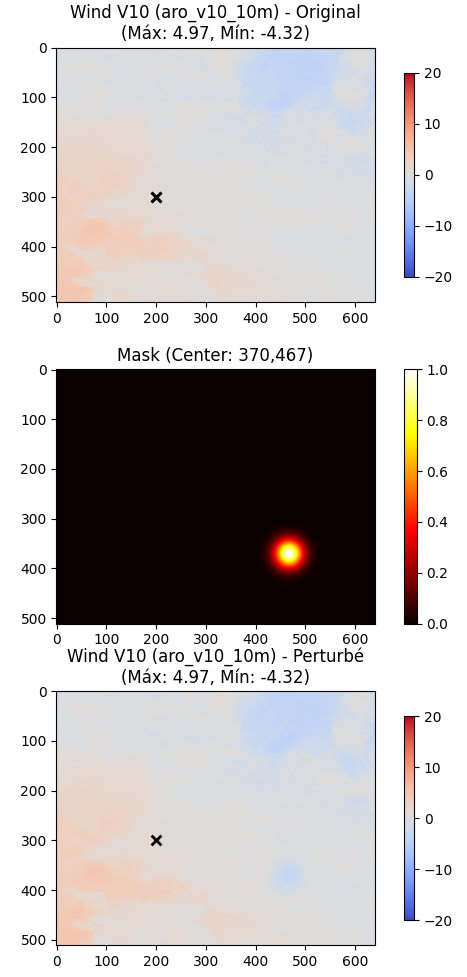
\includegraphics[width=\textwidth]{Images/titan_rain_perturbations/perturbed_c_v10_10m.png}
        \caption{Channel aro\_v10\_10m}
        \label{fig:titan_perturbed_aro_v10}
    \end{subfigure}
    \caption{Example of counterfactuals of Titan image channels from 18/11/2023}
    \label{fig:titan-rain-perturbations}
\end{figure}

Thus, we implemented a loop to generate $K$ counterfactuals for each prediction, balancing time and computational cost with the need for a sufficient number of counterfactuals to produce solid results.

The following configurations were used for generating the anchors:
\begin{itemize}
    \item Sampling period: November 2023.
    \item Number of counterfactuals: $K = 300$.
    \item Center of target location: Centered on $(i, j)$.
    \begin{itemize}
        \item Spatial extent of the center of the perturbation mask: $\sigma_d = 150$ pixels.
    \end{itemize}
    \item Center of perturbation mask: Centered on $(\widehat{i_k}, \widehat{j_k})$.
    \begin{itemize}
        \item Spatial extent of the perturbation mask: $\sigma_e = 20$ pixels.
    \end{itemize}
    \item Prediction difference threshold: $\epsilon = 0.05$ (i.e., the prediction is considered to have changed if it varies by more than 5\%).
\end{itemize}

In each loop, we generate $\widehat{i_k}, \widehat{j_k}, \widehat{c_k}, \widehat{v_k}$ to perturb the image using Eq. \ref{eq:anchor-perturbation}. We then use the generated $z_k$ as an input to obtain the prediction $g_{i,j,c,R}(f(z_k))$ and subsequently calculate $\text{prec}(A)$ using Eq. \ref{eq:extended-prec-anchors}.

The code for this approach was developed in a fork of the py4cast library and can be found in the GitHub repository \cite{py4cast-xai}.

We conducted three tests to compare the results, choosing points with approaching or nearby cloud cover.
Figure \ref{fig:titan-rain-anchors-16} shows the results of the test conducted on $16^{th}$ November data, for the target location $(i, j) = (200, 300)$ (near the region of Chateaubriant).
Figure \ref{fig:titan-rain-anchors-18} shows the results of the test conducted on $18^{th}$ November data, also for the target location $(i, j) = (200, 300)$.
Figure \ref{fig:titan-rain-anchors-21} shows the results of the test conducted on $21^{st}$ November data, for the target location $(i, j) = (300, 250)$ (near the region of Limoges).

\begin{figure}[h]
    \centering
    \begin{subfigure}[b]{0.49\textwidth}
        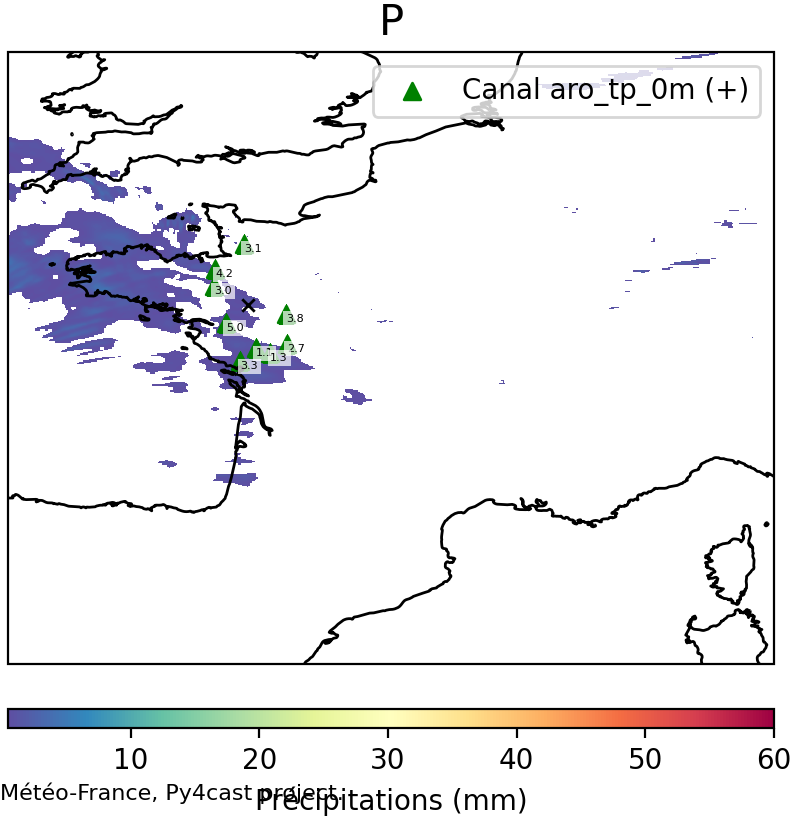
\includegraphics[width=\textwidth]{Images/titan_rain_anchors/nov-16/2023111600_feature_aro_tp_0m.png}
        \caption{Channel aro\_tp\_0m}
    \end{subfigure}
    \hfill
    \begin{subfigure}[b]{0.49\textwidth}
        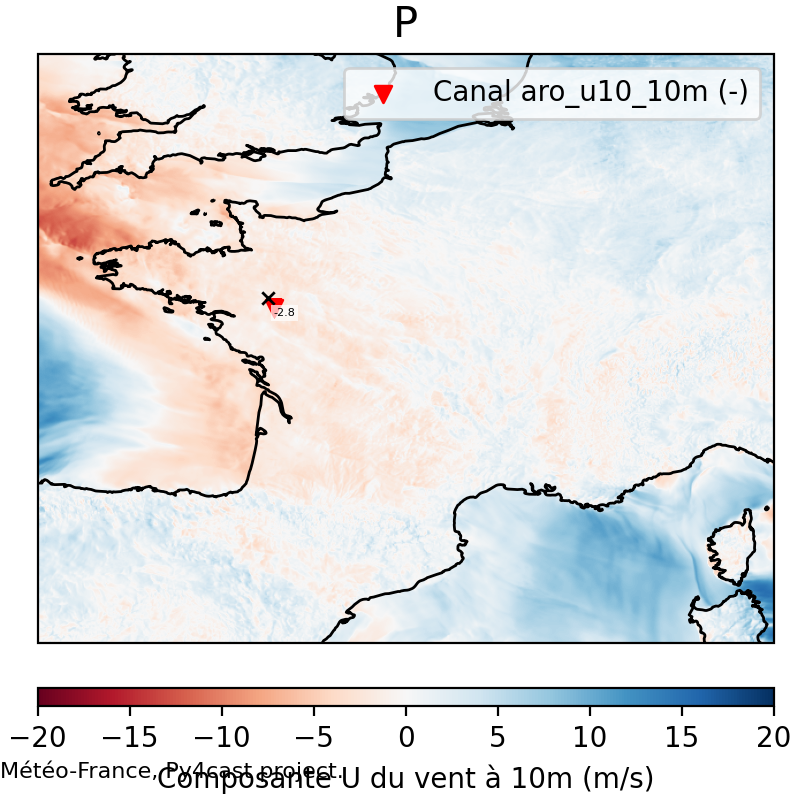
\includegraphics[width=\textwidth]{Images/titan_rain_anchors/nov-16/2023111600_feature_aro_u10_10m.png}
        \caption{Channel aro\_u10\_10m}
    \end{subfigure}
    \hfill
    \begin{subfigure}[b]{0.49\textwidth}
        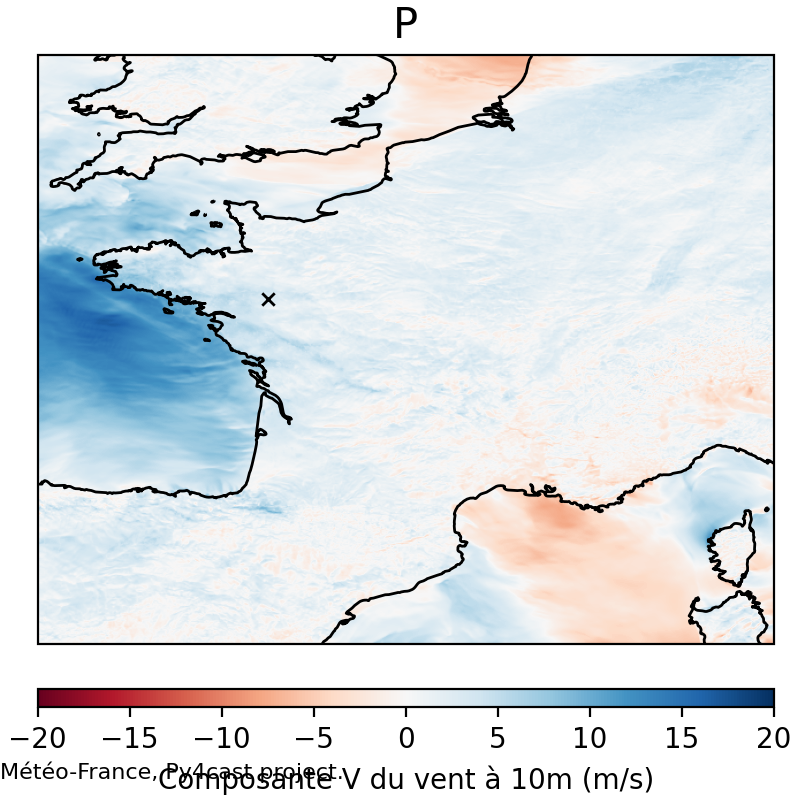
\includegraphics[width=\textwidth]{Images/titan_rain_anchors/nov-16/2023111600_feature_aro_v10_10m.png}
        \caption{Channel aro\_v10\_10m}
    \end{subfigure}
    \caption{Example of anchors applied on "rain" channels, on $16^{th}$ November data.}
    \label{fig:titan-rain-anchors-16}
\end{figure}

\begin{figure}[h]
    \centering
    \begin{subfigure}[b]{0.49\textwidth}
        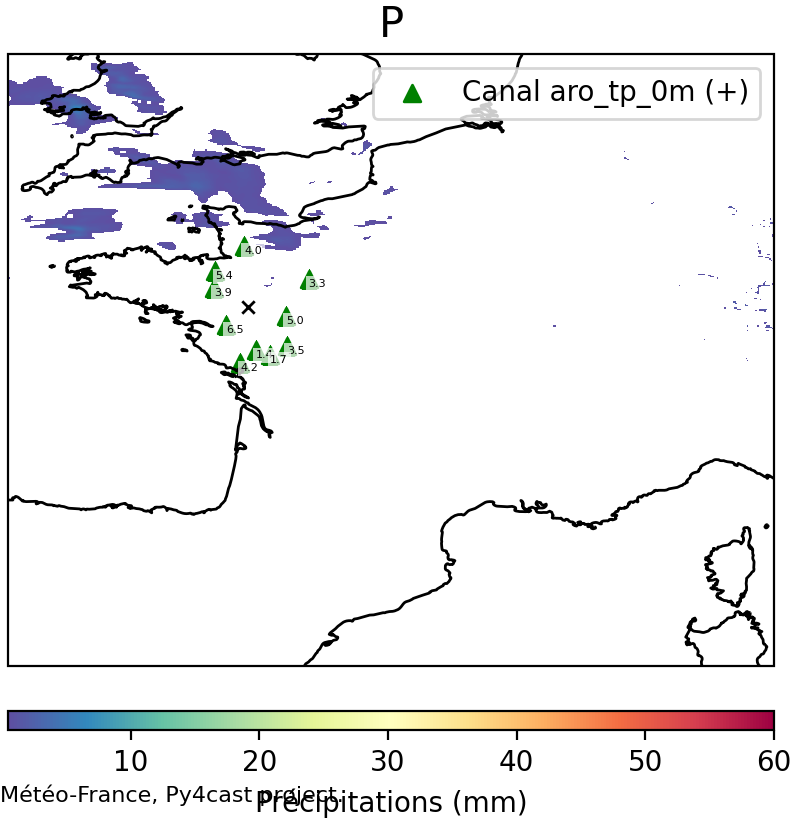
\includegraphics[width=\textwidth]{Images/titan_rain_anchors/nov-18/2023111800_feature_aro_tp_0m.png}
        \caption{Channel aro\_tp\_0m}
    \end{subfigure}
    \hfill
    \begin{subfigure}[b]{0.49\textwidth}
        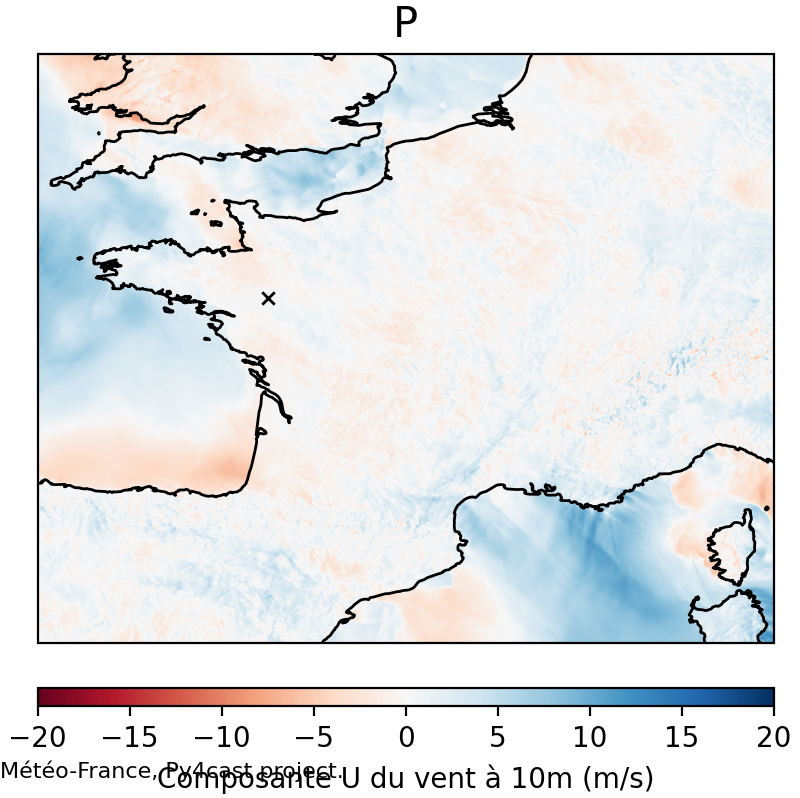
\includegraphics[width=\textwidth]{Images/titan_rain_anchors/nov-18/2023111800_feature_aro_u10_10m.png}
        \caption{Channel aro\_u10\_10m}
    \end{subfigure}
    \hfill
    \begin{subfigure}[b]{0.49\textwidth}
        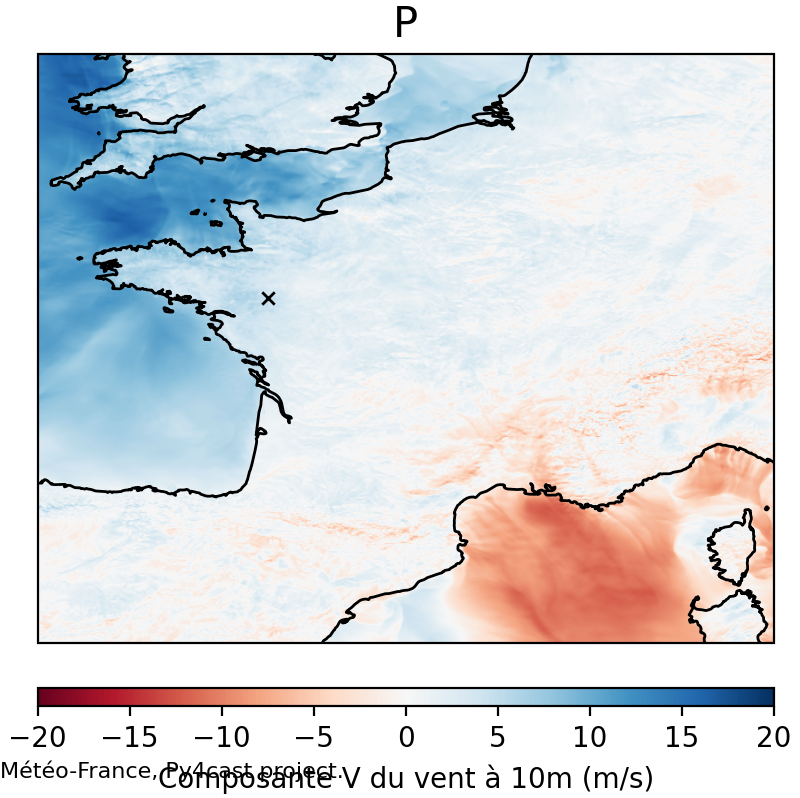
\includegraphics[width=\textwidth]{Images/titan_rain_anchors/nov-18/2023111800_feature_aro_v10_10m.png}
        \caption{Channel aro\_v10\_10m}
    \end{subfigure}
    \caption{Example of anchors applied on "rain" channels, on $18^{th}$ November data.}
    \label{fig:titan-rain-anchors-18}
\end{figure}

\begin{figure}[h]
    \centering
    \begin{subfigure}[b]{0.49\textwidth}
        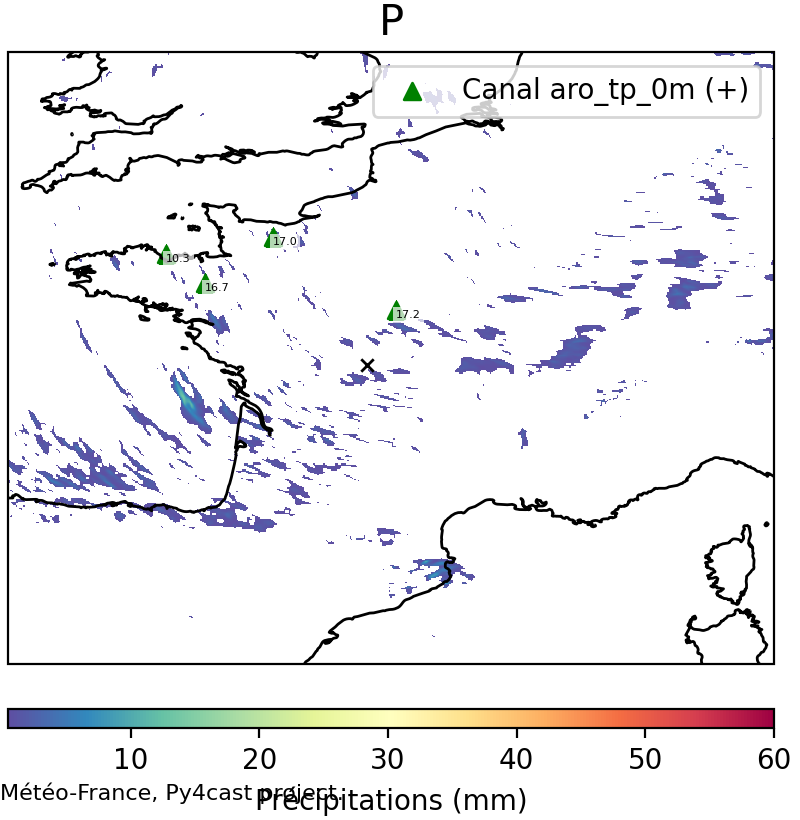
\includegraphics[width=\textwidth]{Images/titan_rain_anchors/nov-21/2023112100_feature_aro_tp_0m.png}
        \caption{Channel aro\_tp\_0m}
    \end{subfigure}
    \hfill
    \begin{subfigure}[b]{0.49\textwidth}
        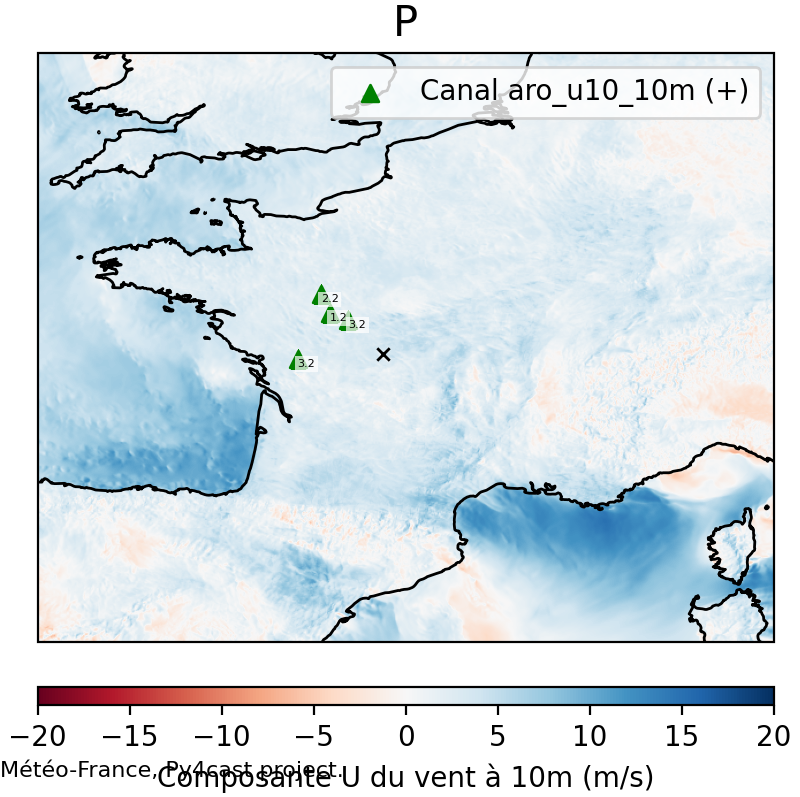
\includegraphics[width=\textwidth]{Images/titan_rain_anchors/nov-21/2023112100_feature_aro_u10_10m.png}
        \caption{Channel aro\_u10\_10m}
    \end{subfigure}
    \hfill
    \begin{subfigure}[b]{0.49\textwidth}
        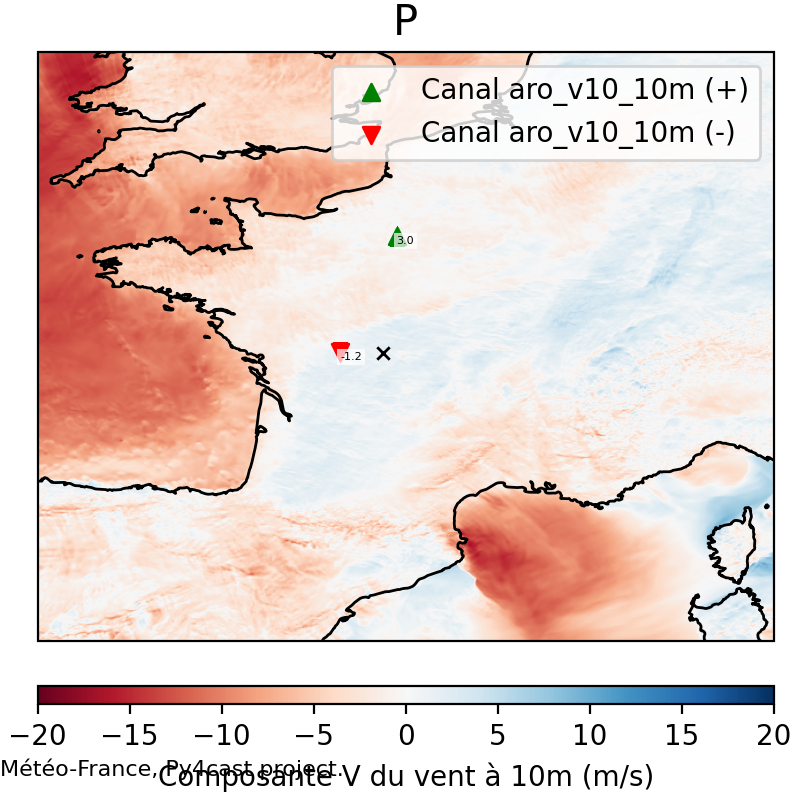
\includegraphics[width=\textwidth]{Images/titan_rain_anchors/nov-21/2023112100_feature_aro_v10_10m.png}
        \caption{Channel aro\_v10\_10m}
    \end{subfigure}
    \caption{Example of anchors applied on "rain" channels, on $21^{st}$ November data.}
    \label{fig:titan-rain-anchors-21}
\end{figure}

The results visually demonstrate how the anchors, marked by the triangle symbols on the plot, are distributed differently in each case.

The first test primarily highlights the \textit{tp\_0m} channel, showing its strong influence on the prediction for the next hour. Conversely, the lack of anchors in the wind channels indicates that no strong wind streams were influencing the region at that time.

The second test shows a scenario similar to the first. It also shows a strong influence of the \textit{tp\_0m} channel due to the approaching clouds and highlights nearby regions that would influence the target area. Additionally, we can associate the anchors in the wind channels with the stronger wind streams coming from the sea.

The third test shows some interesting insights. We chose a point in central France amidst several small concentrations of clouds. The \textit{tp\_0m} channel highlights some regions that could influence the target area, but the anchors are also well distributed across the wind channels. The anchors on the \textit{u10\_10m} and \textit{v10\_10m} channels pinpoint strategic points on the map that are likely to transport precipitation to the region.

In summary, this simplified version of the experiment demonstrates that the Anchors method can effectively describe the influential factors visible in the input images by analyzing each meteorological component.

The first key finding is that Regression Anchors successfully highlight the most influential channels for the prediction at the target location.

The second key finding is that the spatial distribution of the anchor points is coherent with the physical context of each channel and aligns with meteorological principles regarding which features would be expected to change a weather prediction in each case.


% Exportar uma lista de anchors!! para fazer uma tabela e poder analisar